\documentclass{beamer}
\usetheme{focus}

\usepackage{subcaption}
\usepackage[T1]{fontenc}
\usepackage[ngerman]{babel}

\title{Bachelorarbeit\\ Abschlusspräsentation}
\subtitle{Suche von Einzelexemplaren}
\author{Pascal Baumann, Dane Wicki}
\begin{document}
\begin{frame}[plain]
    \maketitle
\end{frame}
\begin{frame}{Einleitung}
\end{frame}
\begin{frame}{Recap Zwischenpräsentation}
\begin{itemize}
    \item Kunde
    \item Referenzimplementation
    \item Konzepte
    \item Herausforderungen
\end{itemize}
\end{frame}
\begin{frame}{Impressionen Zwischenpräsentation}
\begin{figure}
    \centering
    \begin{subfigure}{0.45\linewidth}
        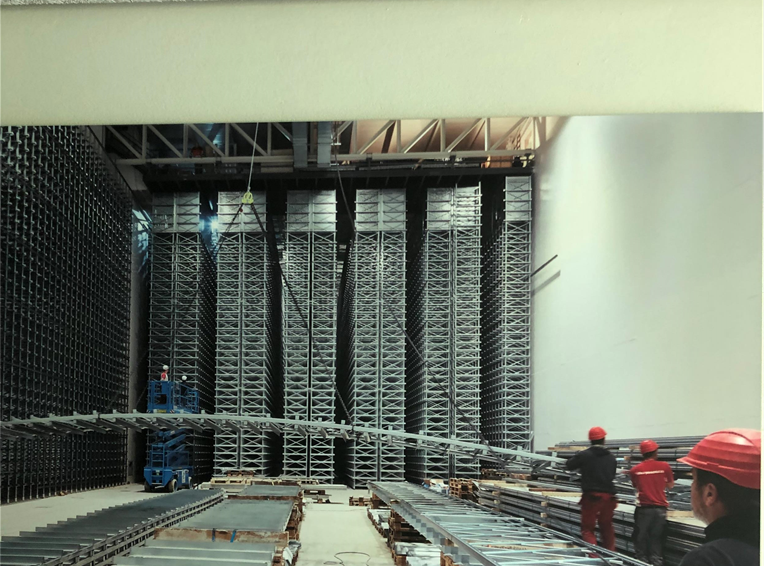
\includegraphics[width=0.8\linewidth]{img/Hochregallager}
    \end{subfigure}
    \begin{subfigure}{0.45\linewidth}
        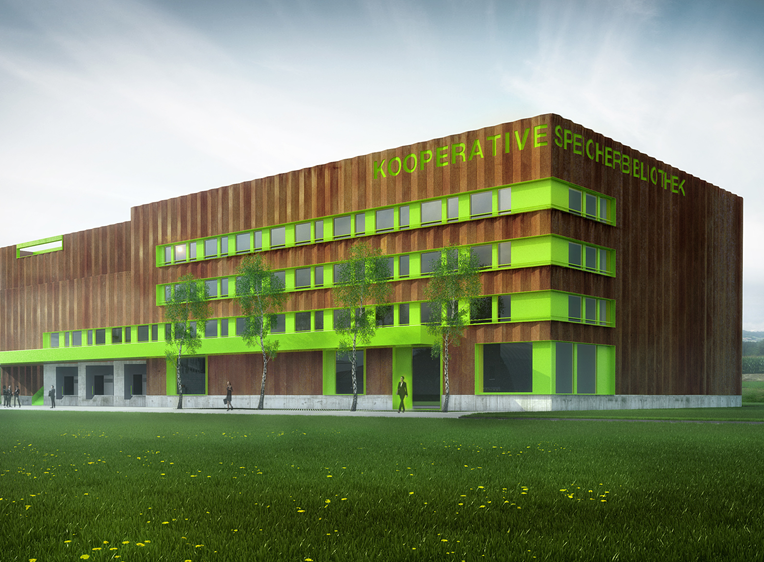
\includegraphics[width=0.8\linewidth]{img/Speicherbibliothek}
    \end{subfigure}
    \vspace{5em}
    \begin{subfigure}{0.7\linewidth}
        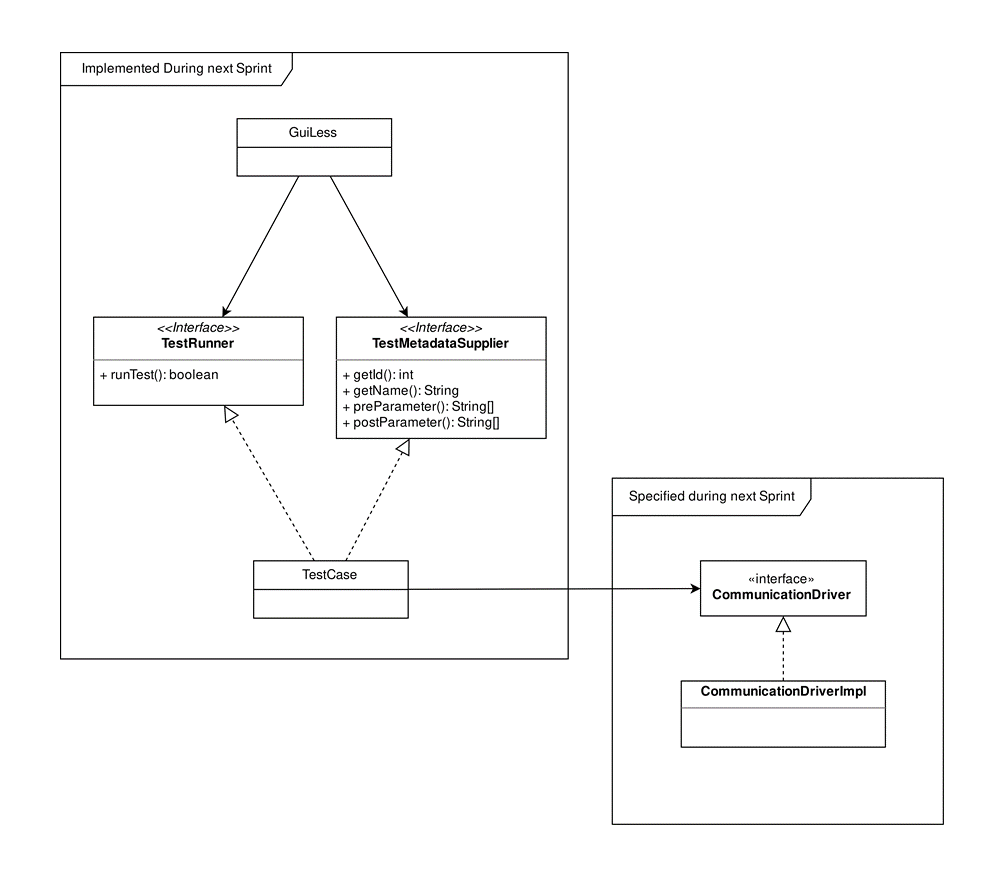
\includegraphics[width=0.7\linewidth]{img/Testframework}
    \end{subfigure}
\end{figure}
\end{frame}
\begin{frame}{Aufgabenstellung}
\centering
\textquotedblleft Klärung Machbarkeit und idealerweise technische Umsetzung zur (teil-) automatischen Suche von Einzelexemplaren im Hochregallager mit RFID.\textquotedblright
\end{frame}
\begin{frame}{Ziele}
Es soll mittels einer Machbarkeitsstudie und einem Proof of Concept untersucht werden, ob es technisch realisierbar ist, Exemplare, welche mit RFID Tags ausgerüstet sind, im Hochregallager der Speicherbibliothek zu finden.
\end{frame}
\begin{frame}{Anforderungen 1/3}
 \begin{itemize}
    \item \textbf{Es sollen mindestens zwei Lösungskonzepte für eine Auswahl der Machbarkeitsstudie entwickelt werden.}
    \item Die Lösungskonzepte müssen auf deren technische Realisierbarkeit untersucht werden.
    \item Es muss mindestens ein entwickeltes Konzept für die Machbarkeitsstudie verwendet werden.
    \item Die Machbarkeitsstudie muss eine Kostenrechnung für die Lösungsansätze beinhalten.
    \item Es soll eine Referenzimplementation entwickelt werden, welche vom Kunde verwendet werden kann.
    
    \item Anforderungen an Konzepte
    \begin{itemize}
        \item Die Lösungskonzepte müssen mit dem Lagersystem kommunizieren können
        \item Die Lösungskonzepte müssen die RFID Tags in weniger als 1 Sekunden identifizieren können.
        \item \textbf{Die Lösungskonzepte müssen für das bestehende Hochregallager der Speicherbibliothek verwendbar sein.}
    \end{itemize}
\end{itemize}
\end{frame}
\begin{frame}{Anforderungen 2/3}
\begin{itemize}
    \item Anforderungen an Proof of Concept
    \begin{itemize}
        \item Das Proof of Concept muss technisch aufzeigen, wie viele RFID Tags in einer Sekunde identifiziert werden können.
    \end{itemize}
    \item Anforderungen an Referenzimplementation
    \begin{itemize}
        \item \textbf{Die Referenzimplementation ist in der Lage die Buch ID eines Exemplares über RFID auszulesen.}
        \item \textbf{Die Referenzimplementation soll erkennen, wenn eine Box ein Exemplar (eines, welches mit RFID ausgestattet ist und technisch auch Lesbar ist) enthält, welches nicht dieser Box zugehörig ist.}
        \item Die Referenzimplementation soll jede erkannte Unstimmigkeit (Exemplar, welches nicht zu diesem Behälter gehört) in einem Logdokument persistieren.
    \end{itemize}
\end{itemize}
\end{frame}
\begin{frame}{Anforderungen 3/3}
\begin{itemize}
    \item ...
    \begin{itemize}
        \item Die Referenzimplementation soll in der Lage sein, dem Endbenutzer, in graphischer Form durch eine Konsolen-Ausgabe, mitzuteilen, welcher Behälter eine Unstimmigkeit enthält.
        \item \textbf{Die Referenzimplementation soll die unter Laborbedingungen erhaltenen Resultate unter Realbedingungen verifizieren.}
        \item \textbf{\textit{Die Referenzimplementation soll mit einer Oracle Datenbank kommunizieren können.}}
    \end{itemize}
 \end{itemize}
\end{frame}
\begin{frame}{Versuche 1/2}
\begin{enumerate}
    \item Versuchsplanung
    \item Versuchsdurchführung und Dokumentation
    \item Auswertung und Erkenntnisse
\end{enumerate}
\end{frame}
\begin{frame}{Versuche 2/2}
\begin{enumerate}
    \item Effektive Reichweite gerade
    \item Lesegeschwindigkeit Bulk Reading
    \item Seitliche Reichweite
    \item Ausrichtung des Tags
    \item Abschirmung durch Gegenstände
    \item Interferenz mehrerer Antennen
    \item Auslesen bewegende Box
    \item Störung durch WLAN
    \item Störung durch Smartphone
    \item Störung durch Kreditkarte
    \item Störung durch Stromquellen
    \item Auslesen von gestapelten Tags
\end{enumerate}
\end{frame}
\begin{frame}{Erkenntnisse aus Versuchen}
\begin{itemize}
    \item 60cm sind harte Grenze
    \item Tags stören sich gegenseitig auf einem relativ grossen Raum
    \item Lesegeschwindigkeit bei mehreren Tags wird exponentiell länger
    \item Auslenkung der Tags problematisch
    \item Abschirmung durch Metall
\end{itemize}
\end{frame}
\begin{frame}{Machbarkeitsstudie}
\begin{itemize}
    \item Recherche zur Durchführung einer Machbarkeitsstudie
    \item Arbeitstrennung auf Kapitelbasis
    \item Kontrolle durch Kunde
    \item Anpassungen auf Wunsch
\end{itemize}
\end{frame}
\begin{frame}{Erkenntnisse aus der Machbarkeitsstudie}
\begin{itemize}
    \item Konzept Zwei (Scanstation) wurde ausgewählt
    \item Konzept ist machbar
    \item Material und Kontakt mit Stöcklin bei Beginn Folgeprojekt
    \item Erstellung verlief soweit ohne Probleme
\end{itemize}
\end{frame}
\begin{frame}{Referenzimplementation}
\begin{figure}[tbh!]
    \centering
    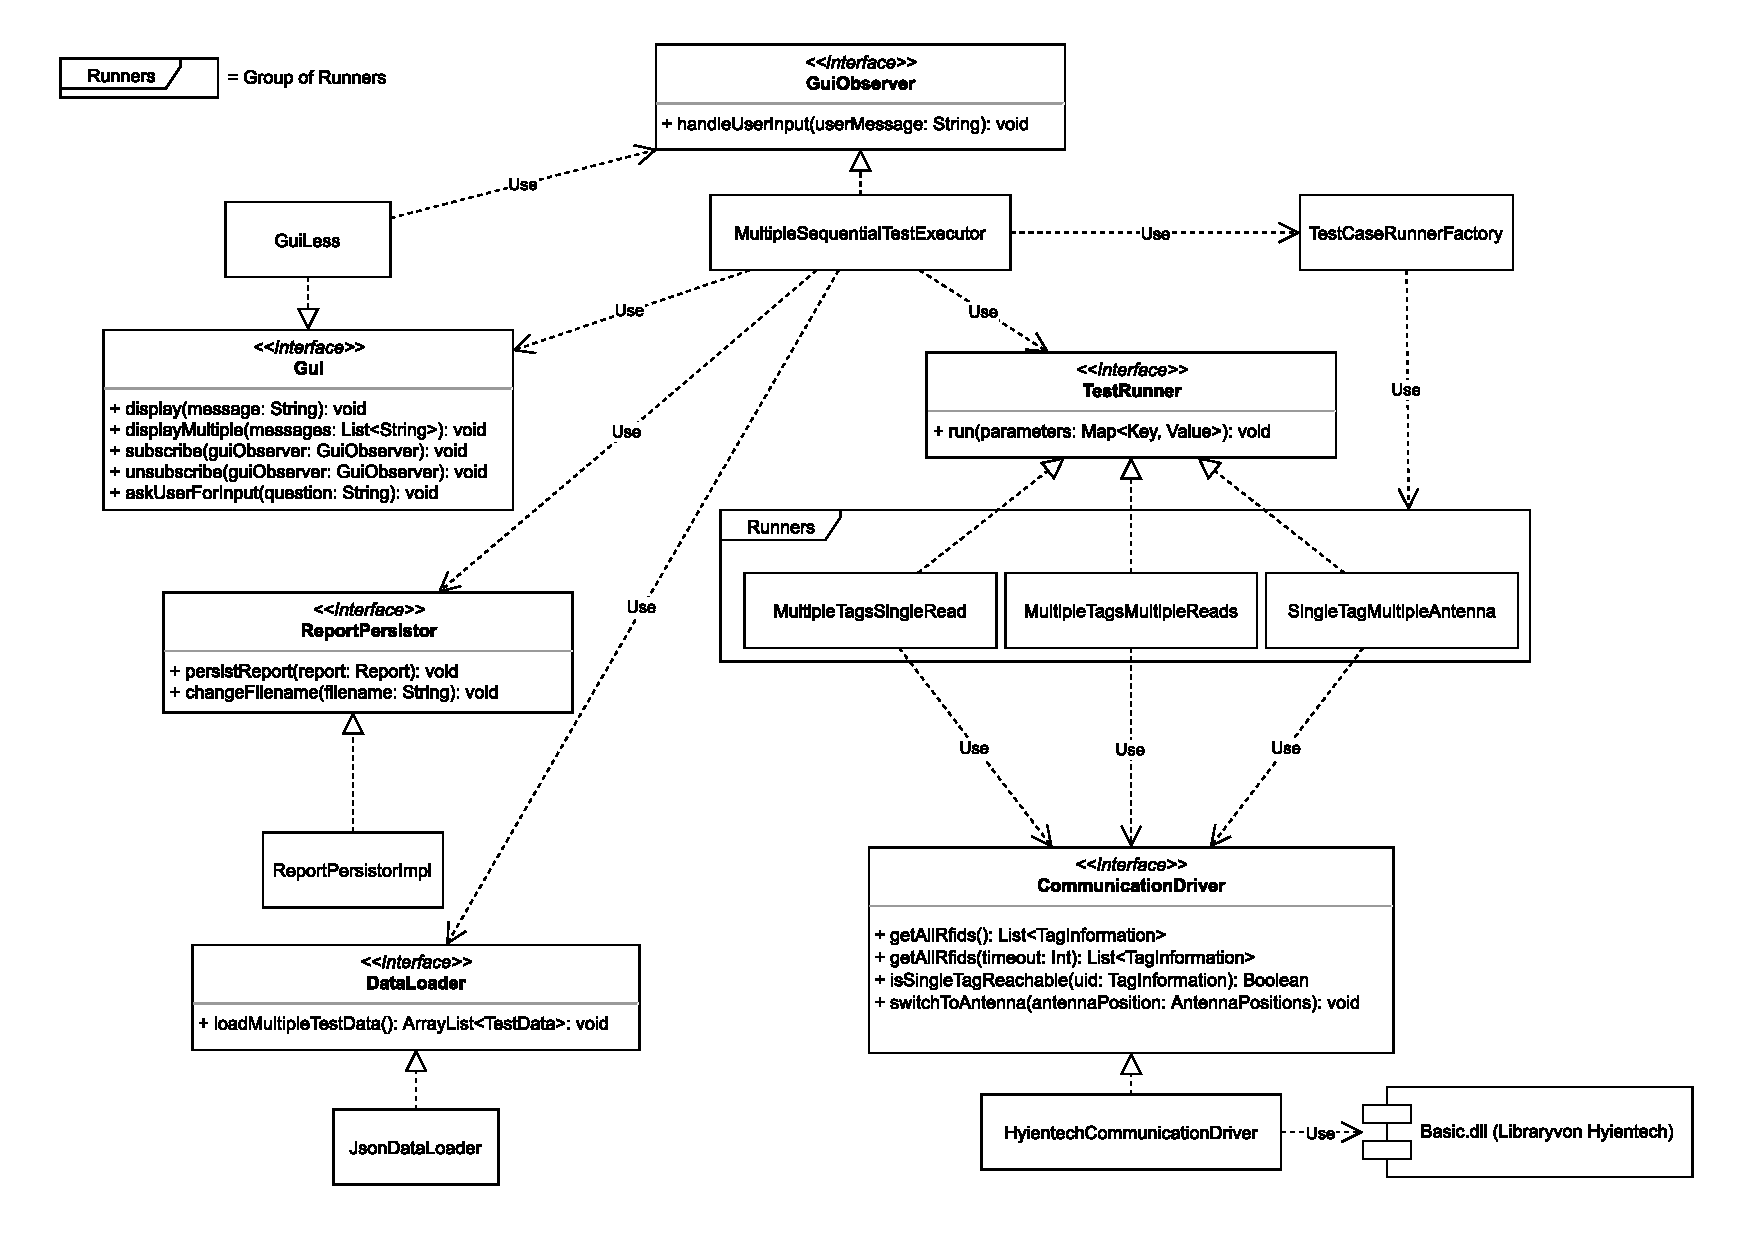
\includegraphics[width=0.8\linewidth]{img/TestApplikation}
    \label{fig:testapplikation}
\end{figure}
\end{frame}
\begin{frame}{Test vor Ort 1/4}
\begin{figure}[tbh!]
    \centering
    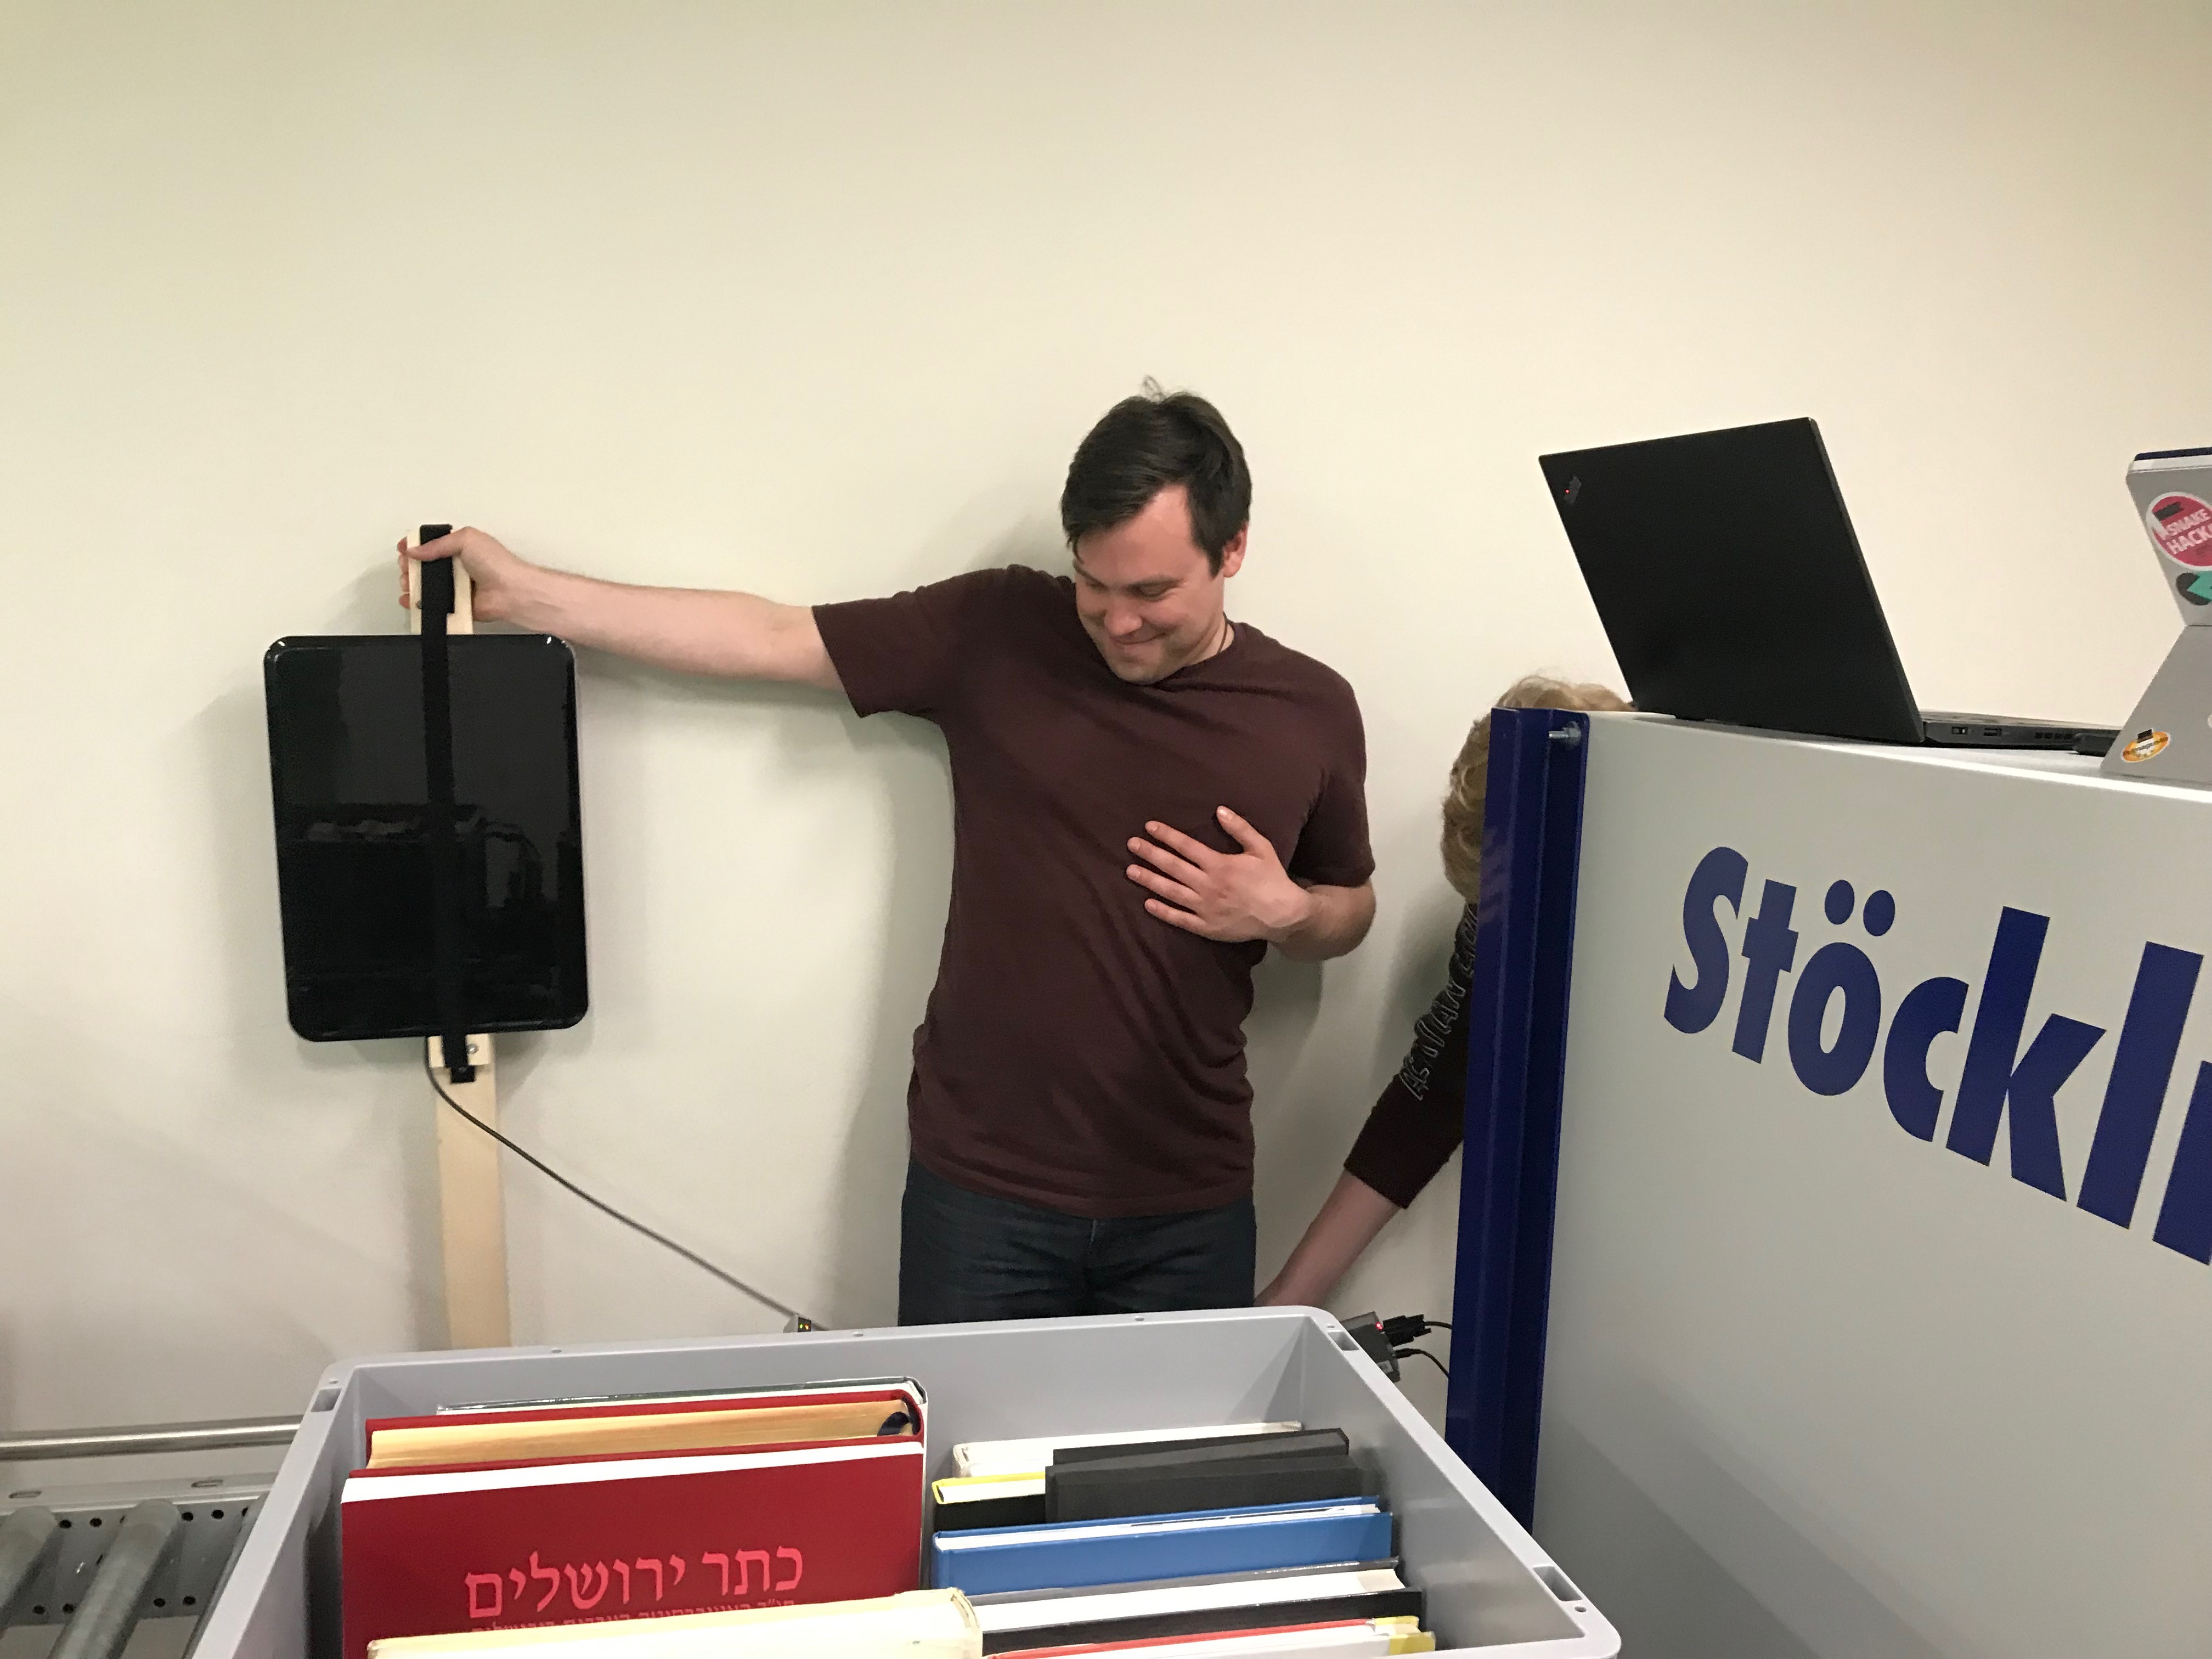
\includegraphics[width=0.8\linewidth]{img/Versuchsaufbau_02}    \label{fig:versuchsaufbau02}
\end{figure}
\end{frame}
\begin{frame}{Test vor Ort 2/4}
\begin{figure}[tbh!]
    \centering
    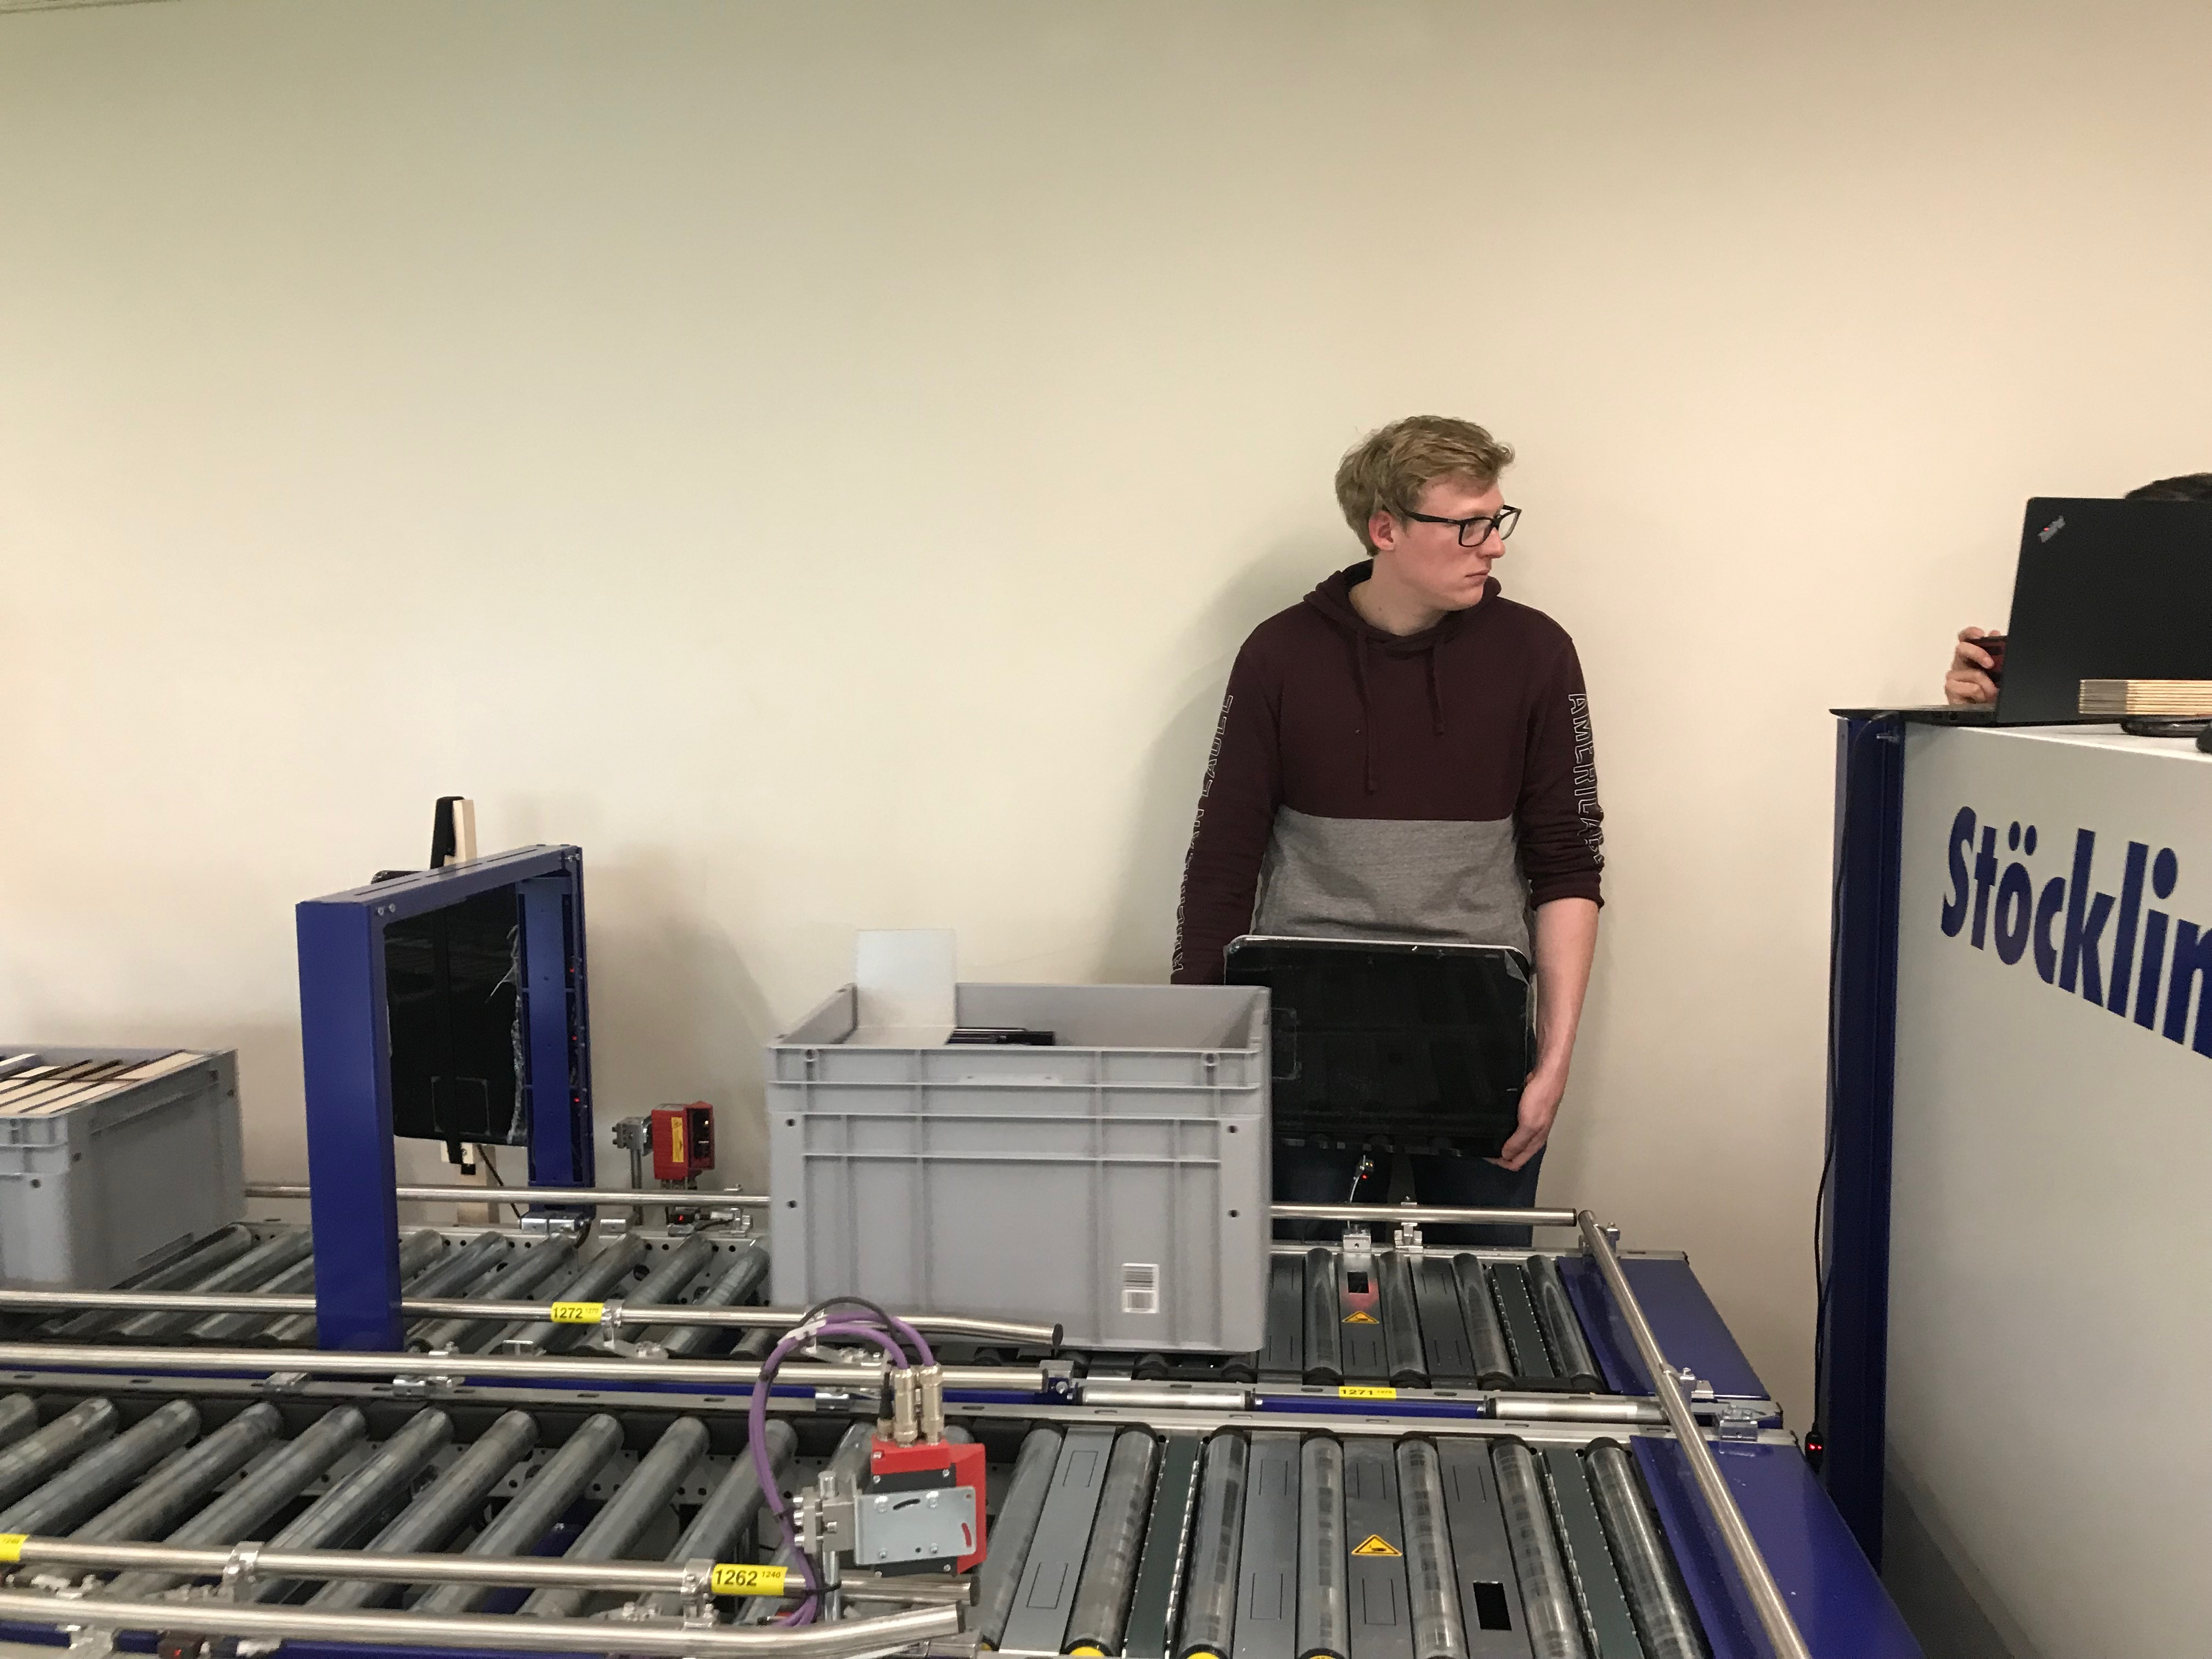
\includegraphics[width=0.8\linewidth]{img/Versuchsaufbau_03}    \label{fig:versuchsaufbau03}
\end{figure}
\end{frame}
\begin{frame}{Test vor Ort 3/4}
\begin{figure}[tbh!]
    \centering
    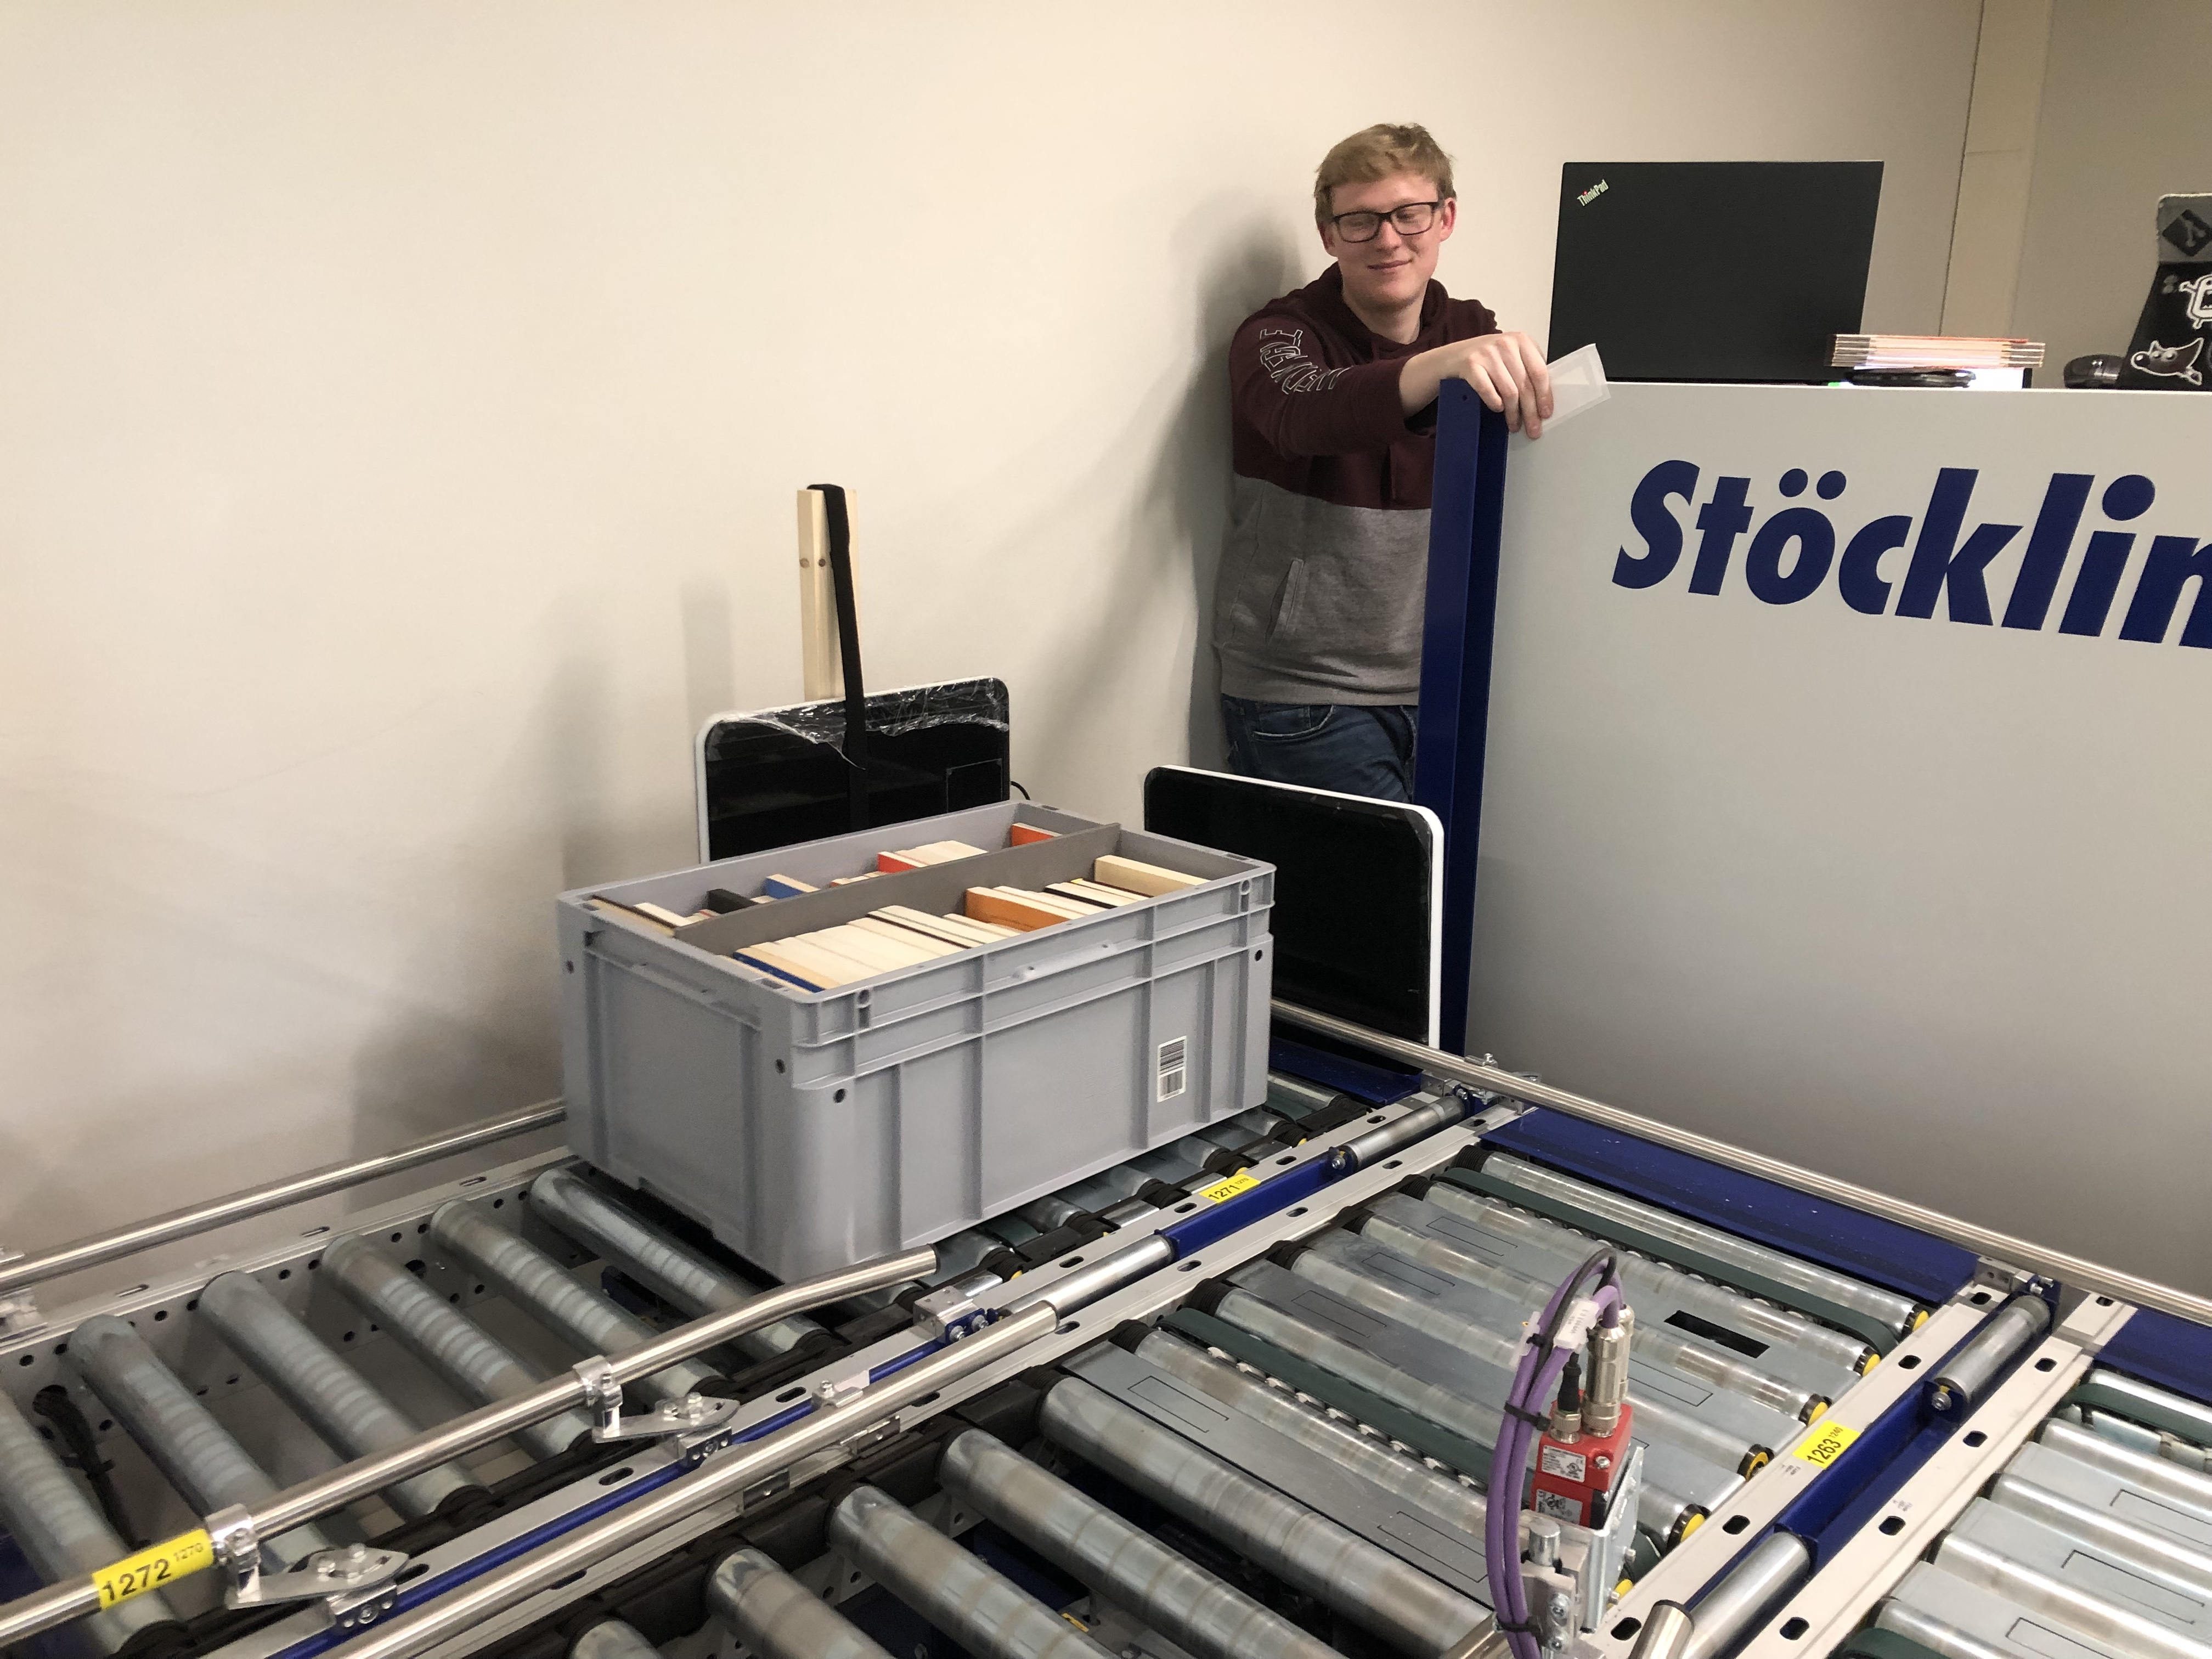
\includegraphics[width=0.8\linewidth]{img/Versuchsaufbau_01}   \label{fig:versuchsaufbau01}
\end{figure}
\end{frame}
\begin{frame}{Test vor Ort 4/4}
\begin{figure}[tbh!]
    \centering
    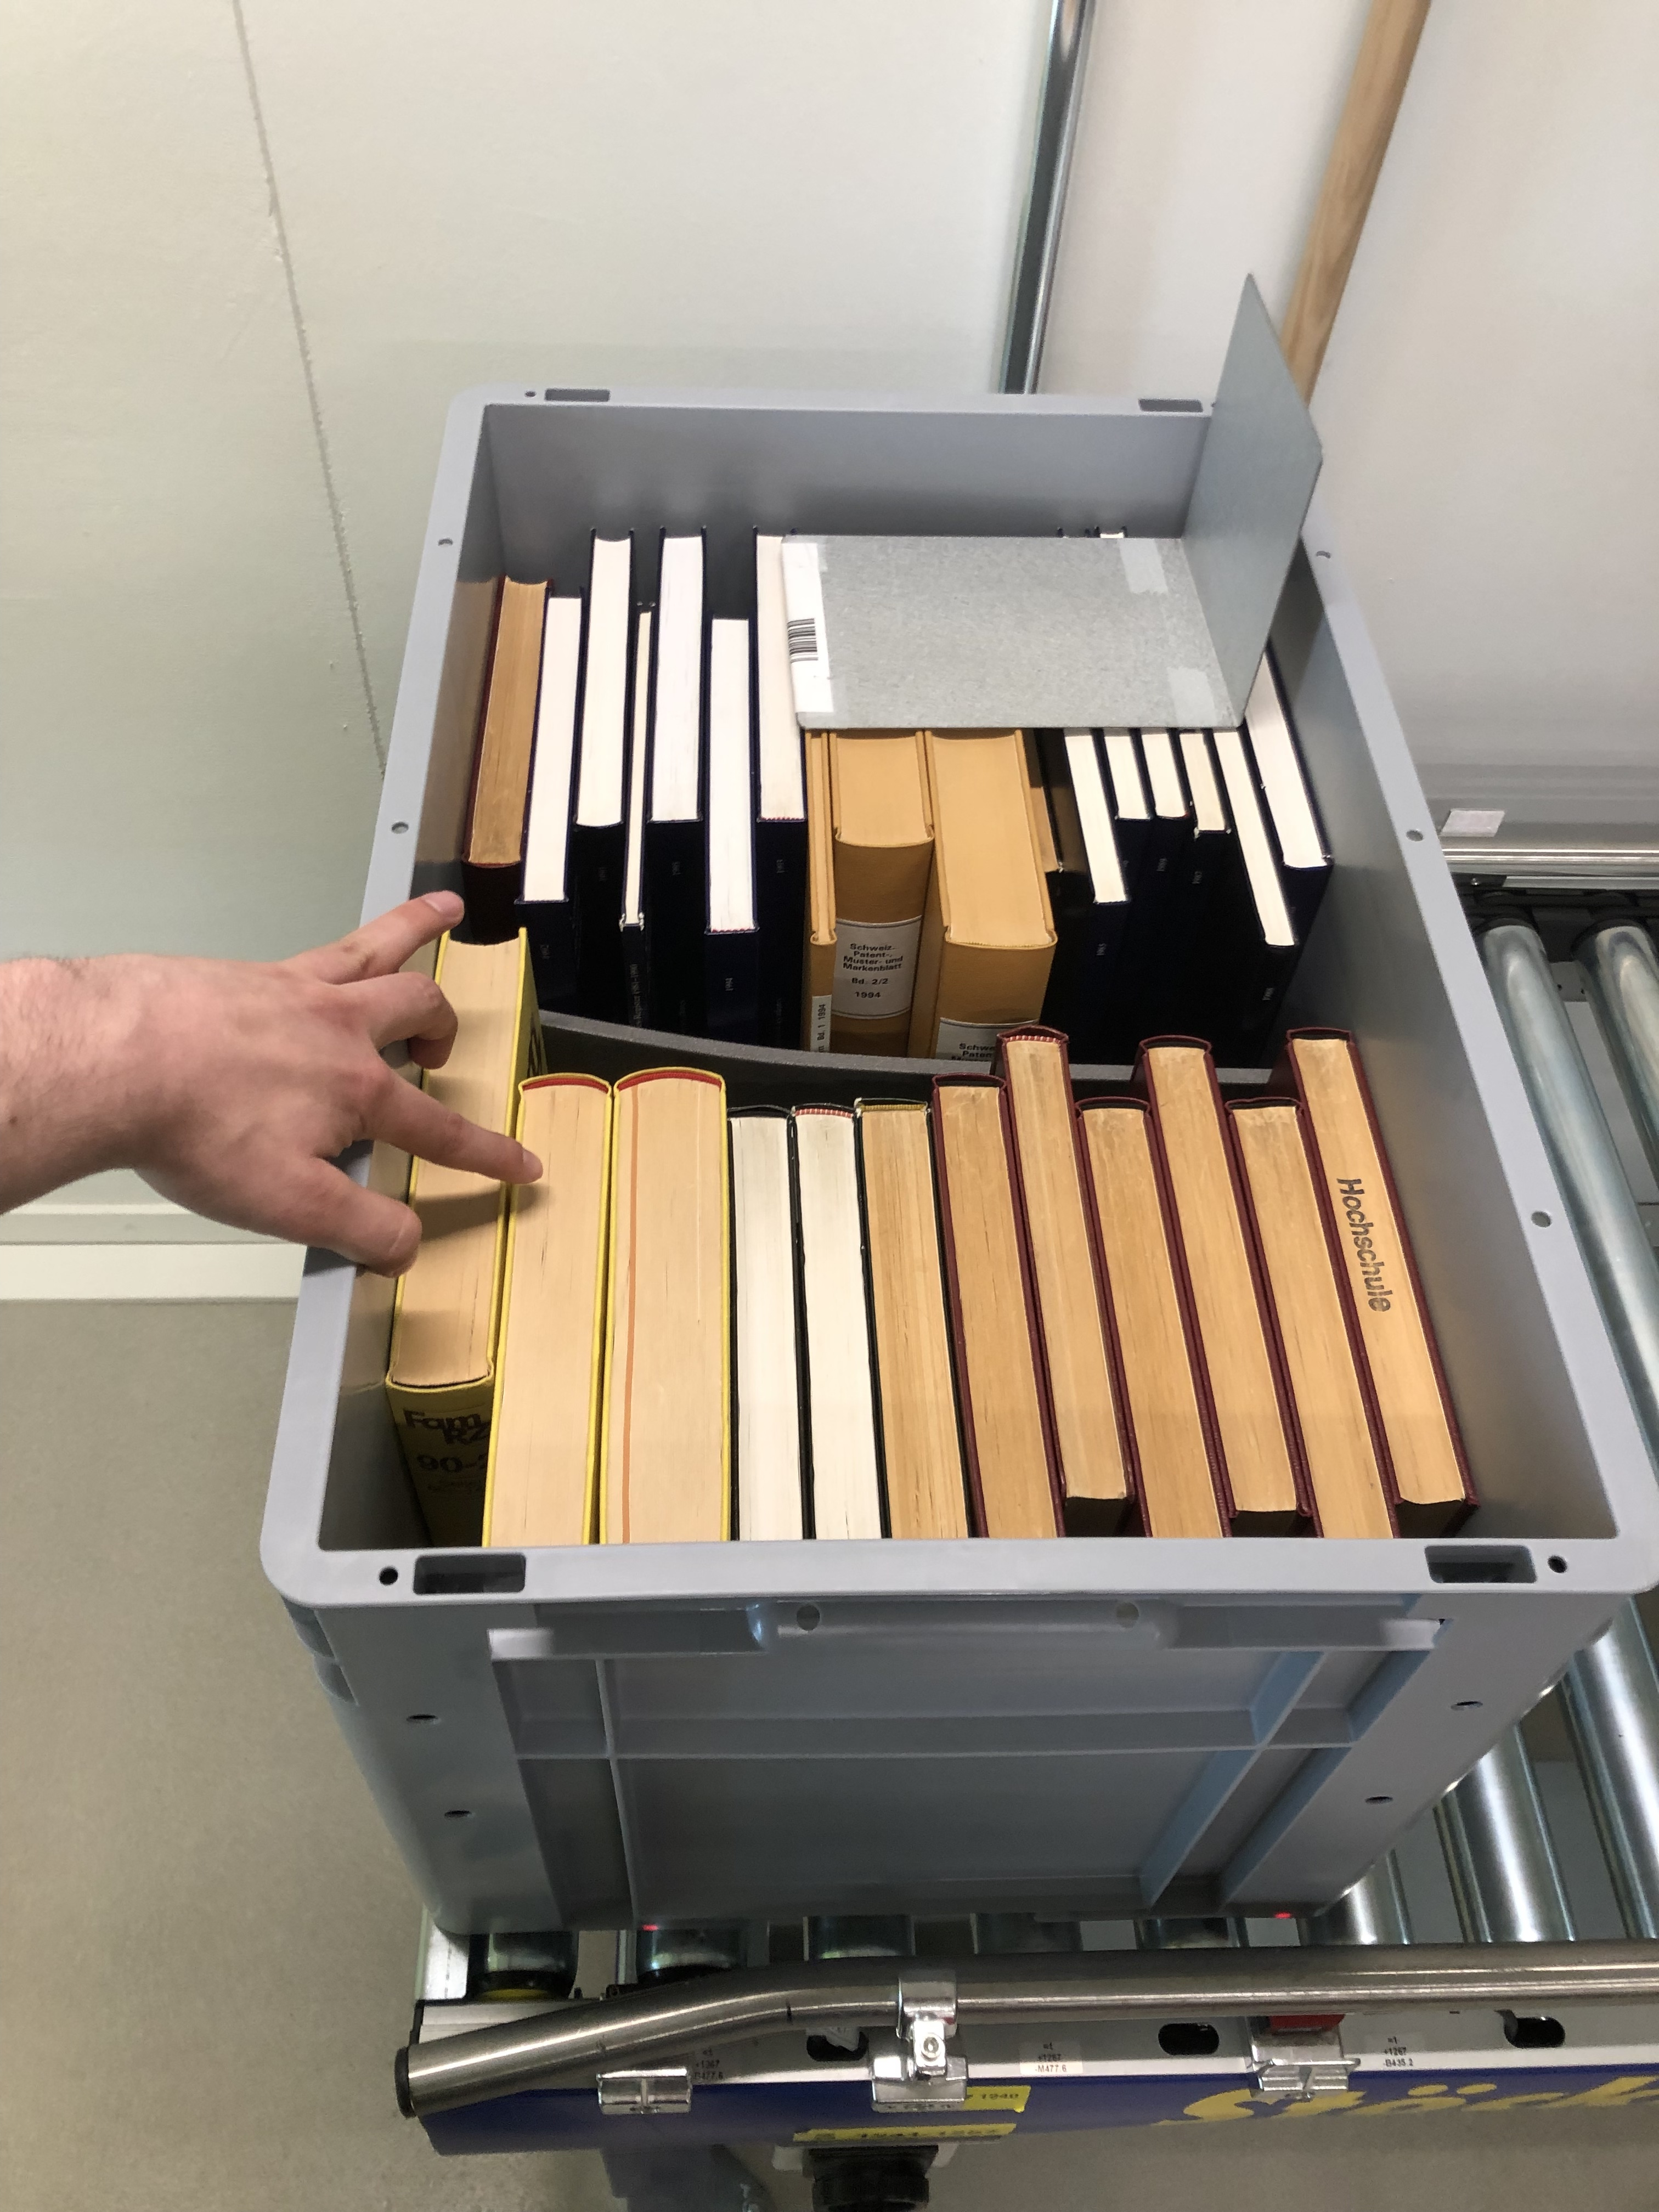
\includegraphics[height=7cm]{img/PositionNichtLesbarerTag}   \label{fig:PositionNichtLesbarerTag}
\end{figure}
\end{frame}
\begin{frame}{Erkenntnisse aus dem Test vor Ort}
\begin{itemize}
    \item Reichweite und Ausrichtungen wichtig
    \item Verarbeitung langsamer als Förderband
    \item Antennenposition macht grossen Unterschied
    \item Abschirmung durch Bücher
\end{itemize}
\end{frame}
\begin{frame}{Projektdokumentation}
\begin{itemize}
    \item CI/CD
    \item Pull Request und Reviews
    \item Viel Fortschritt im letzten Sprint
    \item Feature Complete eine Woche vor Abgabe
\end{itemize}
\end{frame}
\begin{frame}{Allgemeine Herausforderungen}

\end{frame}
\begin{frame}{Vergleich Anforderungen}

\end{frame}
\begin{frame}{Fazit}
\begin{itemize}
    \item Materialbeschaffung
\end{itemize}
\end{frame}
\begin{frame}{Schluss}
\centering
\Large{Danke für die Aufmerksamkeit}\\
\vspace{1em}
\Large{Wir freuen uns auf Ihre Fragen}
\end{frame}
\end{document}
